\documentclass[aspectratio=169]{beamer}

% ======================================
% CONFIGURACIÓN DE LA PLANTILLA UCB
% ======================================

% Cargar el tema personalizado
\usepackage{beamerthemeucb}

% Selección de carrera para configurar colores institucionales:
% Opciones válidas: IMT (Mecatrónica), SIS (Sistemas), INB (Biomédica)
\setcarrera{IMT}

% Paquetes adicionales
\usepackage[spanish]{babel}
\usepackage{array}

% ======================================
% DATOS DE LA PRESENTACIÓN (MODIFICABLES)
% ======================================

% Código y nombre de la materia
\title[IMT-000]{\textbf{IMT-000 \\ Nombre de la asignatura}}

% Nombre del docente
\author{Nombre del docente}

% Correo institucional (usado en portada)
\email{nombre@ucb.edu.bo}

% Instituto o departamento
\institute[UCB]{Nombre del Departamento o Carrera\\
\textbf{Universidad Católica Boliviana San Pablo} \\
\textit{Sede Tarija}}

% Fecha (por defecto: año actual)
\date{\the\year}

% ======================================
% INICIO DEL DOCUMENTO
% ======================================

\begin{document}

% --- PORTADA PERSONALIZADA CON FONDO SUAVE SEGÚN LA CARRERA ---
{
  \setbeamercolor{background canvas}{bg=ucbcoverbg}
  \begin{frame}
    \titlepage
  \end{frame}
}

% --- ÍNDICE AUTOMÁTICO ---
\begin{frame}{Contenido}
  \tableofcontents
\end{frame}

% ======================================
% EJEMPLO DE CONTENIDO ESTRUCTURADO
% ======================================

\section{Sistema de evaluación}
\begin{frame}{Evaluación}
\centering
\scriptsize

% Tabla de evaluación editable según tu sistema
    \begin{table}
        \centering
        \renewcommand{\arraystretch}{3}
        \begin{tabular}{m{4.5cm} m{5.5cm} m{1.5cm}}
            \hline
             \multicolumn{2}{c}{\textbf{Forma de evaluación}} & \textbf{Puntaje}\\
             \hline
             \textbf{Elemento de competencia I}&\begin{minipage}[c]{\linewidth}
            \begin{enumerate}
                \item Prueba de conocimiento
                \item Prueba de ejecución
            \end{enumerate}
        \end{minipage}&35 \\
             \textbf{Elemento de competencia II}&\begin{minipage}[c]{\linewidth}
            \begin{enumerate}
                \item Prueba de conocimiento
                \item Prueba de ejecución
            \end{enumerate}
        \end{minipage}&35 \\
             \textbf{Elemento de competencia III}&\begin{minipage}[c]{\linewidth}
            \begin{enumerate}
                \item Prueba de conocimiento
            \end{enumerate}
        \end{minipage}&30 \\
            \hline
             Final&Productos  &100 \\
             \hline
        \end{tabular}
        \label{tab:evaluacion}
    \end{table}
\end{frame}

% ======================================
% SECCIONES DE CONTENIDO DE CLASE
% ======================================

\section{Unidad 1: Título de unidad}
\begin{frame}{Introducción}
  Breve introducción a la unidad o tema.
\end{frame}

\subsection{Subtema 1.1}
\begin{frame}{Subtema 1.1}
  \begin{itemize}
    \item Punto clave 1
    \item Punto clave 2
  \end{itemize}
\end{frame}

\subsection{Subtema 1.2}
\begin{frame}{Subtema 1.2}
  \begin{itemize}
    \item Definiciones clave
    \item Ejemplos o aplicaciones
  \end{itemize}
\end{frame}

\section{Unidad 2: Otra unidad}
\begin{frame}{Unidad 2}
  Breve descripción de esta unidad.
\end{frame}

\subsection{Subtema 2.1}
\begin{frame}{Subtema 2.1}
  \begin{itemize}
    \item Conceptos relevantes
    \item Aspectos técnicos
  \end{itemize}
\end{frame}

\subsection{Subtema 2.2}
\begin{frame}{Subtema 2.2}
  \begin{itemize}
    \item Aplicaciones prácticas
    \item Observaciones
  \end{itemize}
\end{frame}

% --- IMAGEN DE EJEMPLO (CAMBIAR POR PROPIA) ---
\begin{frame}{Imagen de ejemplo}
  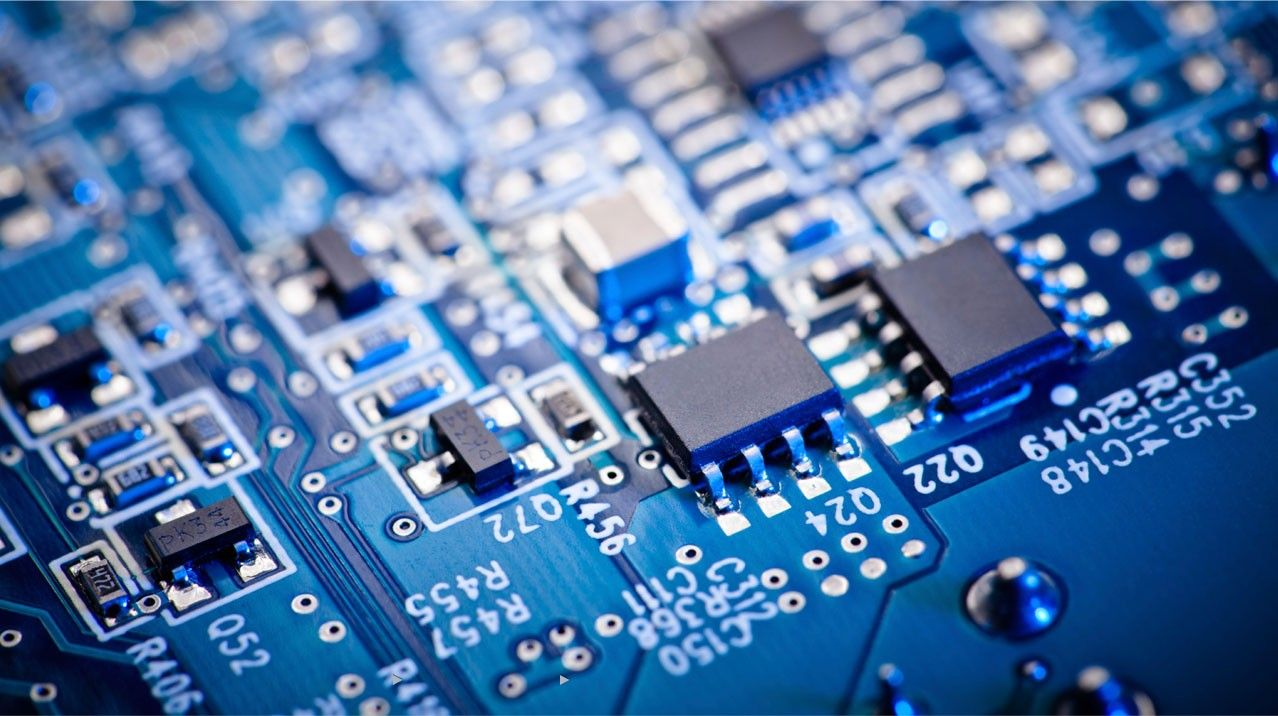
\includegraphics[width=0.8\linewidth]{Images/example-image}
\end{frame}

\section{Unidad 3: Unidad final}
\begin{frame}{Conclusión}
  Conclusión general o reflexiones finales.
\end{frame}

\subsection{Subtema 3.1}
\begin{frame}{Subtema 3.1}
  \begin{itemize}
    \item Tema específico
    \item Relevancia
  \end{itemize}
\end{frame}

\subsection{Subtema 3.2}
\begin{frame}{Subtema 3.2}
  \begin{itemize}
    \item Herramientas o técnicas
    \item Recomendaciones
  \end{itemize}
\end{frame}

% ======================================
% BIBLIOGRAFÍA AUTOMÁTICA DESDE .bib
% ======================================
\begin{frame}[allowframebreaks]{Referencias}
  \nocite{*}  % Muestra todas las entradas del archivo .bib, incluso si no se citan
  \bibliographystyle{plain}
  \bibliography{referencias}
\end{frame}

\end{document}
